\subsection{Récupération via fichiers Excel}
\vspace{1cm}

Heureusement, certaines données étaient disponibles directement sous format Excel. Le traitement de celles-ci était donc beaucoup plus facile que précédemment.

Il m’a simplement fallu placer les fichiers Excel dans un dossier, et définir le bon chemin d’accès à ceux-ci dans mon script. \\

Ensuite en ouvrant un stream du fichier grâce à la fonction \colored{file} , qui renvoie un tableau du contenu, j’ai pu analyser celui-ci grâce à une combinaison des fonctions \colored{array\_map} et \colored{str\_getcsv} pour en tirer un tableau multidimensionnel des lignes du fichier Excel.

Chaque ligne du fichier Excel était sous forme de tableau de chaîne de caractères qu’il fallait ensuite séparer par colonnes, en utilisant le séparateur utilisé dans le fichier.

\begin{figure}[!h]
    \centering
    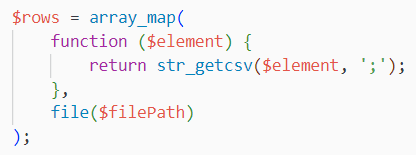
\includegraphics{excel1.png}
    \caption{Parging du fichier Excel}
\end{figure}


Puis en itérant dans chaque ligne de mon fichier, j’ai pu insérer les données voulues dans la base de données en tenant compte de l’encodage des caractères qu’il fallait convertir pour être en accord avec l’encodage de la base de données.


\begin{commentaire}
    Les fichiers Excel sont encodés en \colored{Windows-1252} (ou \colored{CP1252}) et doivent donc être convertis en \colored{UTF-8} pour prendre en compte les caractères accentués par exemple.
\end{commentaire}


\begin{figure}[!h]
    \centering
    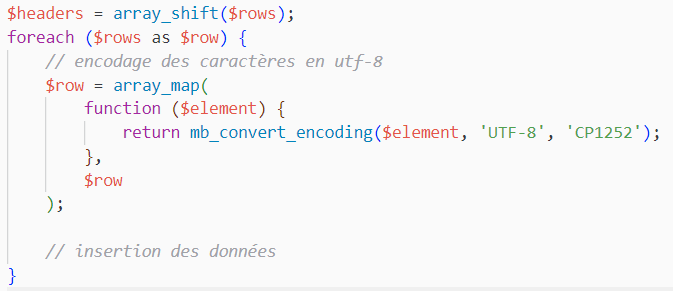
\includegraphics[height=5cm]{excel2.png}
    \caption{Encodage des caractères du fichier}
\end{figure}

\newpage

\subsubsection{Insertion}
\vspace{1cm}

Après avoir récupéré les noms des tables et des colonnes dans \colored{config.json}, j’ai encore une fois utilisé des requêtes préparées et des transactions par soucis de performance et de sécurité.

Les valeurs étant déjà encodées et donc prêtes à être ajoutées à la base de données, j’ai suivi le même principe que pour l’insertion des données via \colored{CURL} , c’est à dire :

\begin{enumerate}
    \item Vérifier si la ligne existe déjà
    \item Si elle existe, alors mettre à jour les données (`UPDATE table`)
    \item Si elle n’existe pas, insérer les données (`INSERT INTO table`)
\end{enumerate}